\section{Testable Predictions and Observational Signatures}
  \label{sec:testable-predictions-and-observational-signatures}

  Before detailing specific observational signatures, it is important to clarify
  the epistemic status of the numerical estimates presented in this section.
  Values such as the $\sim 8$--$10\%$ offset between early- and late-time effective
  determinations of the Hubble constant or the $\sim 10^{-10}\,\mathrm{yr}^{-1}$ drift in effective spacetime observables
  are not proposed as precision predictions.
  They should be understood as order-of-magnitude consistency estimates derived
  from the geometric coupling between the $\chi$ field and the effective relaxation
  fraction $\Omega_\chi$.

  Their role is to demonstrate that the Cosmochrony framework operates within a
  phenomenologically relevant regime, capable of addressing current observational
  tensions without fine-tuning or the introduction of additional dynamical degrees
  of freedom.

  \subsection{Hubble Constant from \texorpdfstring{$\chi$}{χ} Dynamics}
  \label{subsec:hubble-constant-from-chi-dynamics}

  An implication of the relaxation dynamics developed in
  Section~\ref{subsec:emergent-hubble-law} is that, in Cosmochrony,
  the Hubble parameter is not introduced as a free cosmological constant, but arises
  as an effective quantity associated with the irreversible relaxation of the
  $\chi$ substrate.

  At the level of an effective spacetime description, it may be written as
  \begin{equation}
    H(t) = \frac{\dot{\chi}}{\chi},
  \end{equation}
  where the dot denotes differentiation with respect to an effective cosmological
  time parameter introduced solely to parametrize the relaxation ordering, not a
  fundamental temporal evolution.

  In homogeneous regimes, the relaxation rate approaches its maximal admissible
  value.
  Assuming $\dot{\chi}_{\mathrm{eff}} \simeq c$, the present-day Hubble parameter can
  be estimated as
  \begin{equation}
    H_0 \simeq \frac{c}{\chi(t_0)}.
  \end{equation}

  This relation establishes a direct correspondence between the observed Hubble
  constant and the characteristic relaxation scale of $\chi$ at the current epoch.
  Early-universe probes (such as CMB-based inferences) and late-time distance-ladder
  measurements effectively sample $\chi$ at different stages of its relaxation,
  naturally leading to systematically different inferred values of $H_0$ without
  invoking additional cosmological components or fine-tuned initial conditions.

  \paragraph{Resolution of the Hubble tension.}
    The modulation of the $\chi$ relaxation rate by large-scale matter
    inhomogeneities provides a natural mechanism for reconciling early-universe and
    late-time measurements of the Hubble constant.
    Within this framework, the effective Hubble parameter $H(z)$ acquires a mild
    redshift dependence that departs from the $\Lambda$CDM expectation at intermediate
    redshifts ($0.1 \lesssim z \lesssim 10$).
    This deviation reflects the partial projectability of the relaxation dynamics in
    inhomogeneous regimes, rather than the presence of additional cosmological
    components.
    The resulting behavior is directly testable through upcoming baryon acoustic
    oscillation and supernova surveys.

% Requires: \usepackage{pgfplots}
% Optional: \pgfplotsset{compat=1.18}
    \begin{figure}[t]
      \centering
      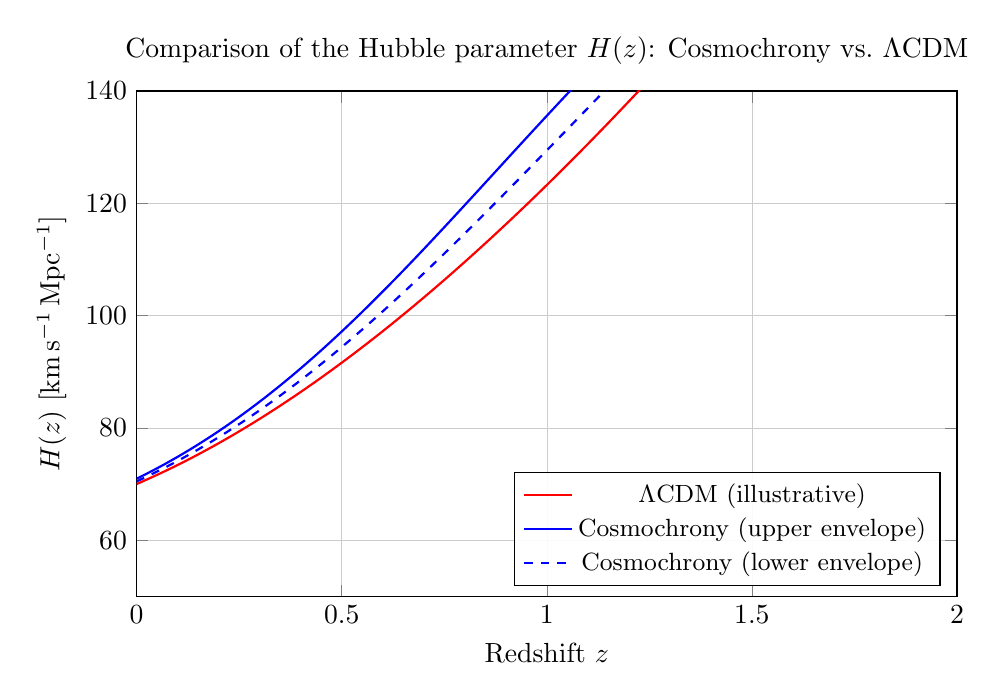
\begin{tikzpicture}
        \begin{axis}[
          width=12cm,
          height=8cm,
          title={Comparison of the Hubble parameter $H(z)$: Cosmochrony vs.\ $\Lambda$CDM},
        xlabel={Redshift $z$},
        ylabel={$H(z)$ [km\,s$^{-1}$\,Mpc$^{-1}$]},
        xmin=0, xmax=2,
        ymin=50, ymax=140,
        xtick={0,0.5,1,1.5,2},
        legend style={
          at={(rel axis cs:0.98,0.02)},
          anchor=south east,
          draw=black,
          fill=white,
          fill opacity=0.9,
          text opacity=1,
          font=\small
        },
        grid=both,
        grid style={line width=.1pt, draw=gray!10},
        major grid style={line width=.2pt, draw=gray!40},
        ]

          % --- Baseline LCDM ---
          \addplot[
            domain=0:2, samples=200,
            red, thick, mark=none
          ]
          {70*sqrt(0.3*(1+x)^3 + 0.7)};
          \addlegendentry{$\Lambda$CDM (illustrative)}

          % --- Cosmochrony band ---
          \addplot[
            domain=0:2, samples=200,
            blue, thick, mark=none
          ]
          {70*sqrt(0.3*(1+x)^3 + 0.7) * (1 + 0.10*exp(-2*(x-1)^2))};
          \addlegendentry{Cosmochrony (upper envelope)}

          \addplot[
            domain=0:2, samples=200,
            blue, thick, dashed, mark=none
          ]
          {70*sqrt(0.3*(1+x)^3 + 0.7) * (1 + 0.05*exp(-2*(x-1)^2))};
          \addlegendentry{Cosmochrony (lower envelope)}
        \end{axis}
      \end{tikzpicture}
      \caption{Schematic comparison of $H(z)$ in Cosmochrony and $\Lambda$CDM.
      Cosmochrony predicts a mild enhancement at intermediate redshifts due to
      relaxation inhomogeneities, providing a discriminating observational test.}
      \label{fig:hubble-comparison}
    \end{figure}

  \subsection{Redshift Drift}
  \label{subsec:redshift-drift}

  An implication of the monotonic relaxation dynamics developed in
  Section~\ref{subsec:expansion-as-relaxation} is that cosmological
  redshifts exhibit a slow temporal evolution when described in an effective
  spacetime parametrization.
  This leads to a redshift drift whose magnitude and redshift dependence differ
  quantitatively from those predicted by the standard $\Lambda$CDM model,
  particularly at intermediate redshifts.

  At the level of an effective parametrization, intended only as an order-of-magnitude
  estimate rather than a derived dynamical law, the effective drift rate may be
  written as
  \begin{equation}
    \dot{z}_{\mathrm{eff}}
    \;\sim\;
    H_0 (1+z) - \frac{c}{\chi(t)},
  \end{equation}
  where the second term reflects the ongoing relaxation of the $\chi$ substrate rather
  than a dark-energy-driven acceleration.
  This corresponds to a secular variation of order
  \[
    \Delta z \sim 10^{-10}\,\mathrm{yr}^{-1}
  \]
  at redshift $z \sim 1$, differing from $\Lambda$CDM expectations at the
  $\sim 10\%$ level in this regime.

  Future high-precision spectroscopic facilities, such as extremely large telescopes
  equipped with ultra-stable spectrographs, may be capable of probing this effect.
  A detection of a redshift drift incompatible with $\Lambda$CDM predictions would
  therefore provide a direct observational discriminator between geometric
  relaxation of the $\chi$ substrate and dark-energy-driven cosmic acceleration.

  \subsection{Gravitational Wave Propagation}
  \label{subsec:gravitational-wave-propagation}

  In the Cosmochrony framework, gravitational waves correspond to propagating
  collective modulations of the $\chi$ field in regimes where a spacetime
  description is applicable.
  They do not constitute independent propagating degrees of freedom, but reflect
  time-dependent redistributions of relaxation constraints within the field.

  In regions of high excitation density, such as near compact objects, the local
  slowdown of $\chi$ relaxation is expected to modify the propagation of these
  modulations.
  In particular, partial decoherence or attenuation may arise due to the coupling
  of propagating modulations to strongly constrained relaxation regions.
  These effects originate from the same collective relaxation constraints
  responsible for gravitational time dilation and horizon formation, and do not
  require the introduction of additional dynamical fields.

  \paragraph{Order-of-magnitude attenuation estimate.}
    Consider a compact object of mass $M$, characterized in effective geometric
    descriptions by a Schwarzschild radius
    \[
      r_s = \frac{2GM}{c^2}.
    \]
    Gravitational-wave modulations of the $\chi$ field propagating through regions
    where the effective relaxation rate is significantly reduced are expected to lose
    coherence through partial redistribution into non-propagating relaxation modes.

    For waves traversing regions within a characteristic distance
    \[
      r \lesssim 10\,\frac{GM}{c^2},
    \]
    the cumulative reduction of effective relaxation conductivity suggests an
    attenuation factor that may be parametrized, at the level of order-of-magnitude
    estimates, as
    \[
      \frac{\Delta A}{A} \sim \mathcal{O}(10^{-2} - 10^{-1}),
    \]
    where the precise magnitude depends on the local $\chi$ correlation length $\xi$
    and on the effective relaxation fraction $\Omega_\chi$ in the vicinity of the
    source.
    This attenuation should be interpreted as a redistribution of wave coherence
    within the $\chi$ relaxation dynamics rather than as dissipative energy loss in
    the conventional field-theoretic sense.

  \paragraph{Observational signature.}
    Such effects are expected to manifest most clearly during the late-time ringdown
    phase of binary black hole mergers, where gravitational-wave signals probe the
    strongly constrained relaxation regime near the effective horizon.
    The resulting signature would appear as a frequency-dependent deviation from
    general relativistic ringdown templates, potentially mimicking anomalous damping
    or mode-dependent quality factors.

    While current ground-based detectors do not yet achieve the signal-to-noise ratios
    required to resolve attenuation at the few-percent level, future space-based
    observatories operating in the LISA band, with expected signal-to-noise ratios
    exceeding $\sim 100$ for massive black hole mergers, may provide sufficient
    sensitivity to test this prediction.

  \paragraph{Semi-quantitative scaling estimate.}
    Within the Cosmochrony framework, attenuation of gravitational-wave amplitudes
    near compact objects arises from the local suppression of $\chi$ relaxation in
    regions of high effective curvature.
    At leading order, the relative amplitude reduction is expected to scale with the
    dimensionless curvature parameter $(r_s / r)$.

    A simple dimensional estimate yields
    \[
      \frac{\Delta A}{A} \sim \left( \frac{r_s}{r} \right)^2 ,
    \]
    indicating that the effect depends explicitly on both the compact object mass and
    the wave trajectory’s impact parameter.
    For propagation at distances $r \approx 10\,r_s$, this scaling gives
    \[
      \frac{\Delta A}{A} \sim 10^{-2},
    \]
    consistent with the order-of-magnitude estimates above and with exploratory
    numerical results obtained from $\chi$-field simulations
    (Appendix~D.3).

  \input{12-predictions/04-spin-and-topological-signatures}
  \subsection{Absence of Dark Energy Signatures}
  \label{subsec:absence-of-dark-energy-signatures}

  Because cosmic acceleration emerges in Cosmochrony as a geometric consequence of
  the global relaxation of the $\chi$ field, no independent dark energy component is
  introduced.
  Accordingly, the framework predicts the absence of signatures associated with
  dynamical dark energy, such as an evolving equation of state, clustering behavior,
  or additional propagating degrees of freedom beyond those already present in the
  effective geometric description.

  Within this perspective, observations consistent with a purely geometric and
  kinematic origin of late-time acceleration would favor Cosmochrony over models
  requiring additional energy components or fine-tuned scalar fields.

  \paragraph{Discriminating observational signatures.}
    The absence of dark energy dynamics cannot be established through any single
    observable.
    Instead, Cosmochrony predicts a correlated pattern of large-scale cosmological
    features reflecting the lack of an inflationary phase and the pre-geometric origin
    of early-time correlations.

    These features include suppressed power at low CMB multipoles, specific angular
    correlations in temperature and polarization, and the absence of an inflationary
    tensor imprint at large angular scales.
    It is the combined presence of these signatures—rather than any individual
    parameter—that provides a potential observational discriminator with respect to
    standard inflationary and dark-energy-driven cosmological models.

  \input{12-predictions/06-emergent_phenomenology}
  \subsection{Summary}
  \label{subsec:summary-predictions}

  Cosmochrony yields a set of observationally testable phenomenological signatures
  across cosmology, gravitation, and quantum phenomena.
  While these features remain compatible with current observations, the framework
  generically allows for correlated departures from standard predictions that may
  become accessible to future high-precision measurements.

  Taken together, these signatures provide concrete avenues for empirical scrutiny.
  The confirmation or falsification of any subset of them would directly constrain
  the viability of Cosmochrony as a physical framework.

